\documentclass[11pt, a4paper]{article}

% --- Packages ---
\usepackage[utf8]{inputenc} % Encoding
\usepackage{amsmath, amssymb, amsthm} % Advanced math typesetting
\usepackage{physics} % Useful commands for physics (derivatives, vectors, braket)
\usepackage{graphicx} % For including diagrams and images
\usepackage{geometry} % Page margins
\usepackage{siunitx} % For proper formatting of SI units
\usepackage{fancyhdr} % Custom headers and footers
\usepackage{xcolor} % For blocks of color
\usepackage{enumitem} % For enumerated lists with letters
\usepackage{float} % For figure strict positioning
\usepackage{parskip} % Remove the indentation and add space between paragraphs

% --- Page Setup ---
\geometry{top=2.5cm, bottom=2.5cm, left=2.5cm, right=2.5cm}
\pagestyle{fancy}
\fancyhf{} % Clear all default header and footer fields
\fancyhead[L]{\textbf{José Carlos López Henestrosa}}
\fancyhead[R]{Inteligencia artificial - PEC2}
\fancyfoot[C]{\thepage} % Page number at the bottom center

% --- Custom Environments ---
\newenvironment{problem}[1][Cuestión]{
	\vspace{0.5cm}
	\noindent{\Large\bfseries #1} \par\vspace{0.5cm}
}{
	\vspace{0.5cm}
}

\begin{document}

	% --- Title Block ---
	\begin{center}
		\Large{ \textbf{PEC2} } \\
		\vspace{0.5cm}
		\normalsize{\textbf{Nombre:} José Carlos López Henestrosa} \\
		\vspace{0.5cm}
		\normalsize{Declaro que ostento la autoría total y llena de todas las tareas que se llevan a cabo en el presente documento. Soy la única persona que ha elaborado cada ejercicio. No he compartido los enunciados con nadie y la única ayuda que he recibido ha sido a través del aula de la UOC y su profesorado y he citado de forma explícita los recursos externos que he usado en la preparación de la PEC.} \\
		\vspace{0.5cm}
		\normalsize{Todas las referencias académicas en esta entrega hacen referencia al libro \textit{Sistemas basasdos en el conocimiento} de los recursos de esta asignatura, salvo que se cite otra fuente explícitamente.}
	\end{center}

	\vspace{1cm}
	\hrule
	\vspace{1cm}

	% --- Exercise 1 ---
	\begin{problem}[Problema 1 (40 \%)]
		Supongamos que se está diseñando un sistema de marcos para clasificar diferentes tipos de vehículos. Este sistema debe permitir recoger toda la información relevante sobre cada vehículo.

		Sabemos que algunas características de vehículos son:

		\begin{itemize}
			\item \textbf{Modelo del vehículo:} por ejemplo, "Tesla Model 3", "Toyota Prius", "Ford F-150".
			\item \textbf{Fabricante:} Empresa que produce el vehículo (Tesla, Toyota, Ford, etc.).
			\item \textbf{Tipo de vehículo:} Puede ser de pasajeros o comercial.
			\item \textbf{Garantía:} Años de garantía del vehículo.
			\item \textbf{Seguridad:} Valoración de seguridad (1 a 5 estrellas).
		\end{itemize}

		Los vehículos se clasifican en los siguientes grupos: \textbf{Vehículos de combustible (ICE), Vehículos eléctricos (BEV), Vehículos híbridos (HEV) e híbridos enchufables (PHEV).} Los vehículos que no son de combustión disponen de batería.

		\textbf{En los vehículos que disponen de bateria, es importante conocer la capacidad de la batería} (medida en kWh) y su \textbf{autonomía} (distancia que puede recorrer el vehículo). Los vehículos eléctricos se caracterizan por el tipo de carga, que puede ser estándar, rápida o ultrarrápida.

		Algunos vehículos tienen un grado de conducción autónoma variable (de 0 a 5). Cada vehículo pertenece a una \textbf{única} categoría principal según su tipo de propulsión.

		\begin{enumerate}[label=\alph*)] 
			\item \textbf{(3 puntos)} Diseñe un sistema de marcos que permita representar el conocimiento que acabamos de describir. Detalle lo máximo posible las clases, subclases, instancias, campos de miembro, campos propios, herencias simples y múltiples, demonios, etc. Además, realice una representación gráfica.
			\item \textbf{(1 punto)} Defina dos instancias e indique qué campos tendrían y de dónde los heredarían.

			{ \color{blue} 
				\begin{figure}[H]
					\centering
					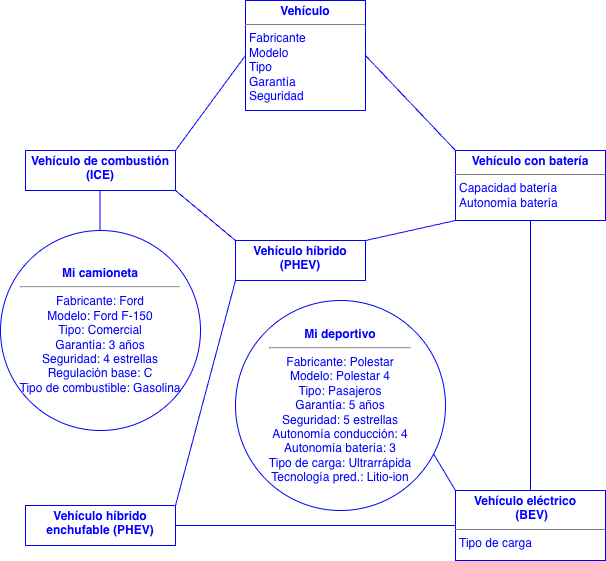
\includegraphics[width=13cm]{imagenes/1_sistema_de_marcos.png}
					\caption{Representación gráfica del sistema de marcos para vehículos.}
				\end{figure}

				\subsection*{Clases}

				\begin{itemize}
					\item \textbf{Clase raíz de la jerarquía: \texttt{Vehículo}}
						\begin{itemize}
							\item \textit{Superclase:} Ninguna.

							\item \textit{Campos miembro:} 
								\begin{itemize}
									\item \textbf{Fabricante (cadena):} Empresa que produce el vehículo.
									\item \textbf{Modelo (cadena):} Nombre del modelo del vehículo.
									\item \textbf{Tipo de vehículos (cadena):} "Pasajeros" o "comercial".
									\item \textbf{Garantía (entero):} Años de garantía.
									\item \textbf{Seguridad (entero):} De 1 a 5.
									\item \textbf{Autonomía de conducción (entero):} De 0 a 5.
								\end{itemize}

							\item \textit{Demonios:}
								\begin{itemize}
									\item \texttt{IF-ADDED} en \textit{Seguridad}: Verifica que el valor introducido esté comprendido entre 1 y 5.
									\item \texttt{IF-ADDED} en \textit{Autonomía de conducción}: Verifica que el valor introducido esté comprendido entre 0 y 5.
									\item \texttt{IF-ADDED} en \textit{Tipos de vehículos}: Verifica que el valor introducido es "Pasajeros" o "Comercial".
								\end{itemize}
						\end{itemize}

					\item \textbf{Subclase 1: \texttt{Vehículo de combustión (ICE)}}
						\begin{itemize}
							\item \textit{Herencia:} Simple (hereda de \texttt{Vehículo}).
							\item \textit{Campos propios:} 
								\begin{itemize}
									\item \textbf{Regulación base (cadena):} Normativa de emisiones estándar (ej. "B", "C", etc.)
									\item \textbf{Tipo de combustible (cadena):} "Gasolina", "Diésel"
								\end{itemize}
						\end{itemize}

					\item \textbf{Subclase 2: \texttt{Vehículo con batería}}
						\begin{itemize}
							\item \textit{Herencia:} Simple (hereda de \texttt{Vehículo}).
							\item \textit{Campos de miembro heredados:} Fabricante, Modelo, Tipo de vehículo, Garantía, Seguridad, Autonomía de conducción.
							\item \textit{Campos de miembro específicos:} 
								\begin{itemize}
									\item \textbf{Capacidad de batería (entero):} Capacidad total de la batería.
									\item \textbf{Autonomía de batería (entero):} Distancia que puede recorrer el vehículo con la batería completamente cargada.
								\end{itemize}
							\item \textit{Campos propios:} 
								\begin{itemize}
									\item \textbf{Tecnología predominante (cadena):} "Litio-ion", "sólida", etc.
								\end{itemize}
							\item \textit{Demonios:}
								\begin{itemize}
									\item \texttt{IF-REMOVED} en \textit{Capacidad de batería}: Borra el valor de Autonomía de batería para evitar que el marco muestre datos inconsistentes.
								\end{itemize}
						\end{itemize}

					\item \textbf{Subclase 3: \texttt{Vehículo híbrido (HEV)}}
						\begin{itemize}
							\item \textit{Herencia:} Múltiple (hereda de \texttt{Vehículo de combustión (ICE)} y de \texttt{Vehículo con batería}).
							\item \textit{Campos de miembro heredados:} Fabricante, Modelo, Tipo de vehículo, Garantía, Seguridad, Autonomía de conducción, Capacidad de batería, Autonomía de batería.
						\end{itemize}

					\item \textbf{Subclase 4: \texttt{Vehículo eléctrico (BEV)}}
						\begin{itemize}
							\item \textit{Herencia:} Simple (hereda de \texttt{Vehículo con batería}).
							\item \textit{Campos de miembro específicos:} Tipo de carga (estándar, rápida, ultrarrápida).
							\item \textit{Demonios:}
								\begin{itemize}
									\item \texttt{IF-ADDED} en \textit{Tipo de carga}: Verifica que el tipo de carga introducido sea "estándar", "rápida" o "ultrarrápida".  
								\end{itemize}
						\end{itemize}

					\item \textbf{Subclase 5: \texttt{Vehículo híbrido enchufable (PHEV)}}
						\begin{itemize}
							\item \textit{Herencia:} Múltiple (hereda de \texttt{Vehículo de combustión (ICE)} y de \texttt{Vehículo eléctrico (BEV)}). Permite obtener el motor de combustión y, al mismo tiempo, heredar el \textit{Tipo de carga} de la rama eléctrica.
							\item \textit{Campos de miembro heredados:} Fabricante, Modelo, Tipo de vehículo, Garantía, Seguridad, Autonomía de conducción, Capacidad de batería, Autonomía de batería.
						\end{itemize}
				\end{itemize}

				A continuación, detallamos las dos instancias representadas gráficamente:

				\begin{itemize}
					\item \textbf{Instancia 1: \texttt{Mi camioneta}}
						\begin{itemize}
							\item \textbf{Es instancia de:} \texttt{Vehículo de combustión (ICE)} (hereda de \texttt{Vehículo}).
							\item \textbf{Campos}
								\begin{itemize}
									\item Heredados de \texttt{Vehículo}: 
										\textit{Fabricante} (Ford), \textit{Modelo} (F-150), \textit{Tipo} (Comercial), \textit{Garantía} (3 años), \textit{Seguridad} (4).
									\item Específicos de \texttt{Vehículo de combustión (ICE)}: 
										\textit{Regulación base} (C),
										\textit{Tipo de combustible } (Gasolina),
								\end{itemize}
						\end{itemize}

					\vspace{0.5cm}

					\item \textbf{Instancia 2: \texttt{Mi deportivo}}
						\begin{itemize}
							\item \textbf{Es instancia de:} \texttt{Vehículo eléctrico (BEV)} (hereda de \texttt{Vehículo con batería}, \texttt{Vehículo}).
							\item \textbf{Campos:}
								\begin{itemize}
									\item Heredados de \texttt{Vehículo} (vía \texttt{Vehículo con batería}): \textit{Fabricante} (Polestar), \textit{Modelo} (Polestar 4), \textit{Tipo} (Pasajeros), \textit{Garantía} (5 años), \textit{Seguridad} (5), \textit{Autonomía conducción} (4).
									\item Heredados de \texttt{Vehículo con batería}: \textit{Autonomía batería} (600 km), \textit{Capacidad batería} (100 kWh).
									\item Específicos de \texttt{Vehículo eléctrico (BEV)}: \textit{Tipo de carga} (Ultrarrápida), \textit{Tecnología predominante} (Litio-ion)
								\end{itemize}
						\end{itemize}
				\end{itemize}
			}
		\end{enumerate}
	\end{problem}

	% --- Exercise 2 ---
	\begin{problem}[Problema 2 (30 \%)]
		La base de conocimiento de un sistema basado en reglas contiene las siguientes reglas:

		\begin{itemize}
			\item \textbf{R1:} Si $A \wedge \neg B \rightarrow C$
			\item \textbf{R2:} Si $C \rightarrow D$
			\item \textbf{R3:} Si $D \wedge E \rightarrow F$
			\item \textbf{R4:} Si $A \rightarrow B$
			\item \textbf{R5:} Si $F \rightarrow \neg E$
			\item \textbf{R6:} Si $\neg D \wedge G \rightarrow G$
			\item \textbf{R7:} Si $H \rightarrow A$
			\item \textbf{R8:} Si $C \rightarrow H$
			\item \textbf{R9:} Si $G \rightarrow E$
		\end{itemize}

		Transcurrido el tercer ciclo de iteración en la ejecución de un algoritmo basado en el encadenamiento hacia adelante, la base de hechos es BF3 = { A(1), G(2), C(3) } (donde el número entre paréntesis indica el ciclo en el que se incluyó como verdadero en la base de hechos un determinado hecho y $\neg$ indica la negación de un hecho).

		El método de control del razonamiento consiste en lo siguiente: primero, tiene mayor prioridad aquella regla con subíndice menor; después, tiene mayor prioridad aquella regla con más condiciones en el antecedente (si hay empate, se aplica el criterio anterior); y, finalmente, hay que tener en cuenta que el sistema está dotado de una estrategia de obstinación, de modo que la aplicación de una regla no puede repetirse.

		\begin{enumerate}[label=\alph*)]
			\item \textbf{(1,5 puntos)} Indicar detalladamente cómo evoluciona la ejecución del método de encadenamiento hacia adelante, a partir de la BH obtenida después del tercer ciclo de ejecución (BH3). Mostrar en cada ciclo cuál es el contenido de la BH. ¿Se puede demostrar B?

			{ \color{blue} 
				Para analizar la evolución a partir del cuarto ciclo, primero debemos entender el estado actual. La base de hechos es $BH_3 = \{ A(1), G(2), C(3) \}$. Observando el hecho $C(3)$, podemos deducir que en el ciclo 3 se aplicó la regla \textbf{R1} ($A \wedge \neg B \rightarrow C$), ya que sus antecedentes ($A$ presente y $B$ ausente) se cumplían y tenía el subíndice más bajo. Debido a la estrategia de \textbf{obstinancia}, que impide que una regla ya utilizada vuelva a aplicarse, R1 queda anulada y no volverá a formar parte del conjunto de conflicto.

				\textbf{Ciclo 4:}
				\begin{itemize}
					\item \textbf{Recuperación (CC4):} Se evalúan los antecedentes de las reglas restantes. 
					Las reglas aplicables son: \textbf{R2} (tiene $C$), \textbf{R4} (tiene $A$), \textbf{R6} (tiene $G$ y no tiene $D$), \textbf{R8} (tiene $C$) y \textbf{R9} (tiene $G$). Por lo tanto, $CC_4 = \{ R2, R4, R6, R8, R9 \}$.
					\item \textbf{Refinamiento:} Aplicamos el método de control. El criterio principal es el \textbf{menor subíndice}. La regla ganadora es \textbf{R2}.
					\item \textbf{Ejecución:} Se aplica R2 ($C \rightarrow D$), infiriendo el hecho $D$ en el ciclo 4.
					\item \textbf{Contenido de la BH:} $BH_4 = \{ A(1), G(2), C(3), D(4) \}$.
				\end{itemize}

				\textbf{Ciclo 5:}
				\begin{itemize}
					\item \textbf{Recuperación (CC5):} Ahora que $D$ está en la BH, la condición $\neg D$ de R6 deja de cumplirse. Las reglas aplicables que no han sido anuladas por obstinancia son: \textbf{R4}, \textbf{R8} y \textbf{R9}. Es decir, $CC_5 = \{ R4, R8, R9 \}$.
					\item \textbf{Refinamiento:} La regla con menor subíndice en el conjunto de conflicto es \textbf{R4}.
					\item \textbf{Ejecución:} Se aplica R4 ($A \rightarrow B$), infiriendo el hecho $B$ en el ciclo 5.
					\item \textbf{Contenido de la BH:} $BH_5 = \{ A(1), G(2), C(3), D(4), B(5) \}$.
				\end{itemize}

				Por lo tanto, concluimos que \textbf{sí se puede demostrar B} porque el hecho $B$ es inferido e incorporado a la base de hechos en el ciclo 5 mediante la ejecución de la regla R4.
			}

			\item \textbf{(1,5 puntos)} ¿Cómo cambiaría la ejecución si la prioridad fuera por número de condiciones en lugar del índice?

			{ \color{blue} 
				Este cambio implica aplicar una estrategia guiada por la \textbf{especificidad}, evaluando la cantidad de conjuntandos en el antecedente. Cuantas más condiciones tenga, mayor prioridad. Si hay empate, se resuelve utilizando el subíndice menor. La obstinancia sigue activa.

				Asumiendo el mismo estado inicial $BH_3 = \{ A(1), G(2), C(3) \}$ con R1 ya consumida, la ejecución evoluciona así:

				\textbf{Ciclo 4:}
				\begin{itemize}
					\item \textbf{Recuperación (CC4):} Igual que en el caso anterior, las reglas aplicables son $CC_4 = \{ R2, R4, R6, R8, R9 \}$.
					\item \textbf{Refinamiento:} Se cuentan las condiciones del antecedente de cada regla. R6 tiene dos condiciones ($\neg D$ y $G$), mientras que R2, R4, R8 y R9 solo tienen una. Por lo tanto, gana \textbf{R6}.
					\item \textbf{Ejecución:} Se aplica R6 ($\neg D \wedge G \rightarrow G$). Aunque infiere el hecho $G$ que ya está presente en la base de hechos, la regla se ejecuta y, por obstinancia, queda anulada para futuros ciclos.
					\item \textbf{Contenido de la BH:} $BH_4 = \{ A(1), G(2), C(3) \}$. (El contenido no cambia, pero se consume una regla).
				\end{itemize}

				\textbf{Ciclo 5:}
				\begin{itemize}
					\item \textbf{Recuperación (CC5):} Al no existir cambios en los hechos y estando R6 consumida, $CC_5 = \{ R2, R4, R8, R9 \}$.
					\item \textbf{Refinamiento:} Todas las reglas empatan con 1 condición. Aplicamos el criterio de desempate de menor subíndice, con el que sale Sale elegida \textbf{R2}.
					\item \textbf{Ejecución:} Se aplica R2 ($C \rightarrow D$), infiriendo $D$.
					\item \textbf{Contenido de la BH:} $BH_5 = \{ A(1), G(2), C(3), D(5) \}$.
				\end{itemize}

				\textbf{Ciclo 6:}
				\begin{itemize}
					\item \textbf{Recuperación (conjunto de conflicto - CC6):} R3 ($D \wedge E \rightarrow F$) aún no se cumple porque falta $E$. Quedan en el conjunto de conflicto $CC_6 = \{ R4, R8, R9 \}$.
					\item \textbf{Refinamiento:} Todas tienen 1 condición. Por desempate de menor subíndice, gana \textbf{R4}.
					\item \textbf{Ejecución:} Se aplica R4 ($A \rightarrow B$), infiriendo $B$.
					\item \textbf{Contenido de la BH:} $BH_6 = \{ A(1), G(2), C(3), D(5), B(6) \}$.
				\end{itemize}

				Como conclusión, sabemos que la ejecución cambiaría en que \textbf{se retrasaría un ciclo completo la demostración de B} pasando del ciclo 5 al ciclo 6 porque en el ciclo 4 el sistema da prioridad a R6 por ser más específica, lo cual consume un ciclo de inferencia en deducir el hecho $G$ que ya conocíamos.
			}
		\end{enumerate}
	\end{problem}

	% --- Exercise 3 ---
	\begin{problem}[Cuestión 3 (30 \%)]
		Imagina que tenemos el siguiente sistema basado en reglas:

		\begin{itemize}
			\item \textbf{R1:} Si $A \wedge B \rightarrow D$
			\item \textbf{R2:} Si $E \rightarrow B$
			\item \textbf{R3:} Si $C \rightarrow B$
			\item \textbf{R4:} Si $D \vee F \rightarrow G$
			\item \textbf{R5:} Si $H \rightarrow F$
			\item \textbf{R6:} Si $I \rightarrow E$
			\item \textbf{R7:} Si $A \rightarrow C$
		\end{itemize}

		\textbf{(3 puntos)} Si se sabe que A y H son ciertos, comprueba si se puede demostrar G con encadenamiento hacia atrás. Indica en cada iteración la Base de hechos, las reglas activas y el objetivo. ¿Qué método de resolución de conflictos has aplicado? (Elige uno y explícalo).

		{ \color{blue} 
			Para resolver este problema aplicando el \textbf{encadenamiento hacia atrás}, partimos del objetivo inicial $G$ y buscamos de manera regresiva las reglas que lo infieren, estableciendo sus antecedentes como nuevos subobjetivos a demostrar hasta llegar a los hechos conocidos.

			Se ha aplicado la estrategia de \textbf{Orden textual} combinada con \textbf{Obstinancia} para la gestión de reglas y un orden de izquierda a derecha para los subobjetivos.

			\begin{itemize}
				\item \textbf{Orden textual:} Si existen varias reglas aplicables para un mismo objetivo, denominadas conjunto de conflicto, determina que se aplique primero aquella que aparece antes en la base de reglas. En este caso, la de menor índice (ej. R2 antes que R3).
				\item \textbf{Obstinancia:} Impide que una regla sea aplicada más de una vez, anulándola si ya se ha usado o ha fallado.
			\end{itemize}

			Ahora que tenemos el planteamiento del algoritmo, lo ejecutamos partiendo del estado $BH_0 = \{A, H\}$ como estado inicial de la base de hechos.

			\begin{itemize}
				\item \textbf{Ciclo 1:}
					\begin{itemize}
						\item \textbf{Objetivo:} $G$
						\item \textbf{BH:} $\{A, H\}$
						\item \textbf{Reglas activas (conjunto de conflicto):} $\{R4\}$
						\item \textbf{Acción:} Seleccionamos R4 ($D \vee F \rightarrow G$). Para demostrar $G$, basta con demostrar $D$ o $F$ debido a la disyunción ($\vee$). Evaluando de izquierda a derecha, fijamos el nuevo objetivo en $D$.
					\end{itemize}

				\item \textbf{Ciclo 2:}
					\begin{itemize}
						\item \textbf{Objetivo:} $D$
						\item \textbf{BH:} $\{A, H\}$
						\item \textbf{Reglas activas:} $\{R1\}$
						\item \textbf{Acción:} Seleccionamos R1 ($A \wedge B \rightarrow D$). Al ser una conjunción ($\wedge$), los nuevos subobjetivos son $A$ y $B$. Evaluamos primero $A$.
					\end{itemize}

				\item \textbf{Ciclo 3:}
					\begin{itemize}
						\item \textbf{Objetivo:} $A$
						\item \textbf{BH:} $\{A, H\}$
						\item \textbf{Acción:} Como el hecho $A$ ya pertenece a la base de hechos ($A \in BH$), el subobjetivo se cumple. Pasamos a evaluar el segundo subobjetivo de R1, que es $B$.
					\end{itemize}

				\item \textbf{Ciclo 4:}
					\begin{itemize}
						\item \textbf{Objetivo:} $B$
						\item \textbf{BH:} $\{A, H\}$
						\item \textbf{Reglas activas:} $\{R2, R3\}$
						\item \textbf{Acción:} Aquí se produce un conflicto. Aplicando el \textbf{orden textual}, seleccionamos la regla de menor índice: R2 ($E \rightarrow B$). Establecemos el nuevo subobjetivo en $E$.
					\end{itemize}

				\item \textbf{Ciclo 5:}
					\begin{itemize}
						\item \textbf{Objetivo:} $E$
						\item \textbf{BH:} $\{A, H\}$
						\item \textbf{Reglas activas:} $\{R6\}$
						\item \textbf{Acción:} Seleccionamos R6 ($I \rightarrow E$). Nuevo subobjetivo: $I$.
					\end{itemize}

				\item \textbf{Ciclo 6:}
					\begin{itemize}
						\item \textbf{Objetivo:} $I$
						\item \textbf{BH:} $\{A, H\}$
						\item \textbf{Reglas activas:} $\emptyset$ (Vacío)
						\item \textbf{Acción:} Ninguna regla concluye $I$ y no está en la BH. El subobjetivo $I$ fracasa, haciendo que $E$ y R2 también fracasen. El sistema realiza un \textit{backtracking}) al punto de decisión más reciente con alternativas (ciclo 4).
					\end{itemize}

				\item \textbf{Ciclo 7:}
					\begin{itemize}
						\item \textbf{Objetivo:} $B$ (reanudado)
						\item \textbf{BH:} $\{A, H\}$
						\item \textbf{Reglas activas:} $\{R3\}$ (R2 fue anulada por obstinancia)
						\item \textbf{Acción:} Seleccionamos la alternativa pendiente R3 ($C \rightarrow B$). Nuevo subobjetivo: $C$.
					\end{itemize}

				\item \textbf{Ciclo 8:}
					\begin{itemize}
						\item \textbf{Objetivo:} $C$
						\item \textbf{BH:} $\{A, H\}$
						\item \textbf{Reglas activas:} $\{R7\}$
						\item \textbf{Acción:} Seleccionamos R7 ($A \rightarrow C$). Nuevo subobjetivo: $A$.
					\end{itemize}

				\item \textbf{Ciclo 9:}
					\begin{itemize}
						\item \textbf{Objetivo:} $A$
						\item \textbf{BH:} $\{A, H\}$
						\item \textbf{Acción:} $A$ pertenece a la base de hechos inicial, por lo que el objetivo se cumple.
					\end{itemize}
				\end{itemize}

			Al demostrarse el subobjetivo $A$ en el ciclo 9, se lleva a cabo el razonamiento en cadena hacia arriba:

			\begin{enumerate}
				\item R7 deduce $C$ $\rightarrow$ La BH se actualiza a $\{A, H, C\}$.
				\item R3 deduce $B$ $\rightarrow$ La BH se actualiza a $\{A, H, C, B\}$.
				\item Con $A$ y $B$ confirmados, R1 deduce $D$ $\rightarrow$ La BH se actualiza a $\{A, H, C, B, D\}$.
				\item Como $D$ es verdadero, la disyunción ($D \vee F$) de R4 se cumple, lo cual demuestra la meta principal \textbf{G}.
			\end{enumerate}

			\textit{Nota: Si el orden de evaluación del motor de inferencia hubiese verificado el lado derecho de la disyunción de R4 ($F$) en primer lugar en vez de $D$, el proceso habría sido mucho más directo, ya que el objetivo $F$ activa R5 ($H \rightarrow F$), y como $H \in BH$, habría inferido $F$ y, por consiguiente, el objetivo general $G$ en tan solo 3 iteraciones.}
		}
	\end{problem}
\end{document}